%\documentclass[aps,pre,preprint,groupedaddress,nofootinbib]{revtex4}
\documentclass[aps,pre,preprint,nofootinbib]{revtex4}
%\documentclass[aps,twocolumn,pre,nofootinbib]{revtex4}   % list options between brackets
\usepackage{listings}              % list packages between braces
\usepackage{graphicx}
\usepackage{epstopdf}
%\usepackage{cite}

% type user-defined commands here

\begin{document}

\title{Erlang Term Storage Implementation}
\author{Kjell Winblad and Stavros Aronis}
\date{\today}


\begin{abstract}

  This report describes in detail how the Erlang Term Storage (ETS) is implemented.
  The report is created in the RELEASE project as the first step towards creating a more scalable ETS implementation.
  ETS tables are commonly used to share data between processes in Erlang programs.
  It is important to have a scalable ETS implementation because shared data is often the bottleneck in concurrent applications.
  The main goals of the report are:
  \begin{itemize}
   \item to get an understanding of the current implementation of the different ETS tables
   \item to communicate this knowledge (for example to the Erlang OTP team)
  \end{itemize} 

\end{abstract}

\maketitle

\section{Introduction}

Erlang Term Storage (ETS) is a feature included in the Erlang runtime system.
It supports storage of Erlang tuples in ETS tables which are outside the processes' heaps.
This prevents garbage collection from copying these tuples while collecting memory space from a process' heap and can also be used to efficiently share data between processes. %I don't understand the part about garbage collection
An Erlang ETS table behaves as if a dedicated process serves requests for insertions, lookups and other common operations on a key value dictionary, but is implemented in a more efficient way.
Most of the operations on an ETS table are implemented as built-in functions (BIFs) in the Erlang runtime system. 
An ETS table can be accessed by either a \emph{table identifier} (TID) or an atom (in case of a \emph{named} table).
In either case the identifier for the table is returned by the call to the \verb|ets:new/2| BIF.
The \verb|ets:new/2| BIF can also take a list of options that specify: 

\begin{itemize}
\item 
  The access level for the table which can be \verb|private|, \verb|protected| or \verb|public|.
  See the Erlang documentation for \verb|ets:new| for more information about these options\footnote{http://www.erlang.org/doc/man/ets.html}.
\item
  Whether the table is a \verb|named_table|, in which case the atom provided as a table name can be used instead of the TID in table operations.
\item 
  Whether the table type is \verb|set|, \verb|bag |, \verb|duplicate_bag| or \verb|ordered_set|. 
  See section~\ref{sec:table_types} for information about the data-structures used in the different table types.
\item 
  Whether fine grained and/or faster locking is enabled for read and write operations (specified with the options \verb|write_concurrency| and \verb|read_concurrency|). 
  See section~\ref{sec:concurrency_options} and \ref{sec:benchmark} for more information about these options.
\end{itemize}

ETS tables are owned by the creating process as long as the creating process is alive, unless the ownership has been passed to another process with the \verb|ets:give_away| operation.
If the owner of an ETS table terminates the table will be deleted, unless the \verb|heir| option is set.
Developers can use the \verb|heir| option (only during creation) or the \verb|set_heir| BIF (at anytime) to specify a process that will inherit the table when the current owner terminates. 
If a process has been specified with the \verb|heir| option, it will receive a message signalling the transfer of table ownership, when the previous owner terminates.

\subsection{Overview of Table Operations}

This section gives an overview of the most fundamental ETS table operations. 
See the Erlang documentation for ETS tables for a complete description of all table operations. 
See section~\ref{sec:table_types} for information about the data-structures used in the tables.

\begin{description}
 \item[lookup(Tab, Key) $\rightarrow$ [Object]] 
 Returns a list of objects that have the given key. 
 \item[insert(Tab, ObjectOrObjects) $\rightarrow$ true]
 Insert the given object (or objects, if the parameter is a list of objects) to the table.
 \item[insert\_new(Tab, ObjectOrObjects) $\rightarrow$ true]
 This operation will insert the given object or objects if no object with the same key as any of the object(s) exists. 
 If a key already exists the operation will return false.
 \item[delete(Tab, Key) $\rightarrow$ true] Deletes all objects with the given key from the table.
 \item[first(Tab) $\rightarrow$ Key $|$ \texttt{end\_of\_table} ] Returns the first key in the table. If the table is of the \verb|ordered_set| type, the first key in Erlang term order will be returned. If the table is of any other type, the first key according to the table's internal order will be returned. If the table is empty, \verb|end_of_table| will be returned.
 \item[last(Tab) $\rightarrow$ Key $|$ \texttt{end\_of\_table} ] Returns the last key in the table.
\end{description}

\section{Previous Work}

  Scott Lystig Fritchie has suggested a new implementation of the set table type based on Judy-arrays~\cite{ScottEtsJudy}.
  In this work the performance of a Judy-array based implementation is experimentally compared to the AVL-tree and linear hast table implementations currently available.
  For large table sizes the operations lookup, insert and update seem to be faster with the Judy-array based implementation.
  However, term deletion and table traversal seem to be slower in the Judy-array based implementation.
  The benchmarks in the paper do not test how the implementation performs when operations are performed concurrently.
  
  Patrik Nyblom has suggested the addition of software transactional memory (STM) support for Erlang ETS tables~\cite{PatrikErlangTrans}.
  In this work it is argued that STM support could be added to Erlang with only minor changes to the ETS implementation.
  The suggested implementation would not effect the performance of ETS when the transactional features are not used.
  At the same time it could increase parallelism for use cases where the only alternative without transactional memory support is to serialize all operations on the ETS table (or tables).
  Benchmark results for a prototype of ETS with transactional memory, show that transactional memory support for ETS could make some use cases more scalable with the number of cores.
  

\section{Handling of Tables}

The infrastructure for the handling of tables is described in this section. 
An overview of the data-structures used on a global level is provided in section~\ref{sec:tables_overview}.
How locking is done when tables are accessed concurrently is described in section~\ref{sec:tables_locking}.

\subsection{Global data structures}
\label{sec:tables_overview}

The following data structures are maintained on a system-wide level and are used for ``generic book-keeping''.
Low level operations like finding the main data structure for a specific table or handling ownership trasfers use only these data structures.

\begin{description}
\item[meta\_main\_table]
  Contains pointers to the main data structure of all the tables that exis currently in the system.
  TIDs map to a slot in this table.
\item[meta\_name\_table]
  Contains mappings from the names of named tables to the repective TIDs.
\item[meta\_pid\_to\_tab]
  Maps processes (PIDs) to tables owned by them.
\item[meta\_pid\_to\_fixed\_tab]
  Maps processes (PIDs) to tables that are fixated by them.
\end{description}

\subsection{Locking} \label{sec:tables_locking}

Different levels of locking are required for each operation on an ETS table.
In general, the same lock data structure is used for both read and write on the data protected by the lock and operations request and obtain different levels of access.
For example, acquisition of the lock to read the data should not block other readers but should block all the writers until the lock is released.
Similarly, acquisition of the lock to write on the data should block both readers and writers trying to access the same data.

\begin{itemize}
\item Creation and deletion of a table require the acquisition of the write lock protecting the \verb|meta_main_table|.
\item Creation, deletion and renaming of a named table also require the acquisition of the write lock protecting the \verb|meta_name_table|.
\item Read and write operations on a table require the acquisition of the appropriate table locks.
  Using the default options, each table has just one main lock, used for all entries.
  Depending on the type and the options specified when a table is created, two read and write operations for different keys can be allowed to run in parallel, by locking only parts of the table.
  We give further details in section~\ref{sec:table_types}.
\end{itemize}

\section{Table Types} \label{sec:table_types}

Tables of type \verb|set|, \verb|bag| and \verb|duplicate_bag| do not impose any particular order between their entries.
These tables are implemented in the runtime system as hash tables.
In contrast, \verb|ordered_set| tables have their entries ordered according to their keys and are therefore implemented as AVL trees.
The runtime system is structured in such a way that operations which are transparent to the underlying implementation of a table are handled with normal C functions, while operations that depend on the implementation are dispatched from the equivalent of a method table.

\subsection{Hash tables}

Hash tables distribute their key-value entries to buckets, depending on a hash value generated using the key.

\subsubsection{Fine Locking}

Protected and public hash tables support fine locking if the option \verb|write_concurrency| is provided during creation.
In this case an array of locks is allocated during table creation and each lock protects a subset of the buckets.
The size of the lock array is defined at \emph{compile time} and is currently set to 16.
(Therefore each lock ``protects'' those buckets whose index modulo 16 equals the lock's index.)

\subsubsection{Data Structure}

The current implementation\footnote{All the particular sizes mentioned reflect faithfully the current implementation.} of ETS tables is based on linear dynamic hash tables~\cite{Larson}.
The main data structure is called ``extended segment'' and has two parts:
\begin{enumerate}
  \item A ``bucket'' section, containing 256 pointers to lists of the key-value pairs that belong to the respective bucket.
    These lists correspond to the common ``chaining'' implementation of a hash table.
  \item A ``segment'' section, pointing to ``bucket'' sections.
\end{enumerate}
The runtime system can also allocate plain ``bucket'' sections, without ``segment'' sections attached.
As an invariant, the entry point for all access is a ``current'' extended segment, but there might also exist ``previous'' extended segments that are still used for their bucket sections and may be used again for their segment sections if the table is shrinked.

As an invariant, a continuous range of buckets (starting with bucket 0) is declared as ``active'' buckets.
The index of the highest active bucket is stored as \verb|nactive|.

To operate with some object of the table, the hash value of the key of the object is first calculated.
This hash value is then mapped to the index of a bucket of the table, masking some of the least significant bits of the hash value, depending on the index of the highest active bucket.
If the index obtained through this masking corresponds to a bucket that is active, this is the bucket that should contain the object.
If the bucket is not active, another significant bit is dropped, and the bucket with the resulting index value is used instead.

The bucket id itself can be divided in two parts: a segment address and a bucket offset.
The segment address is first used as an index on the segment section of the current ``extended segment'', to find the base pointer of a bucket section.
Then the bucket offset is used to find the specific bucket in the bucket section.

Under each bucket there exists a chain of hash values that map to it.
Within each such chain there is no ordering of the objects.
New objects are appended at the end of a chain, as we might need to find and overwrite objects with the same key.

\begin{figure}[htb]
\centering
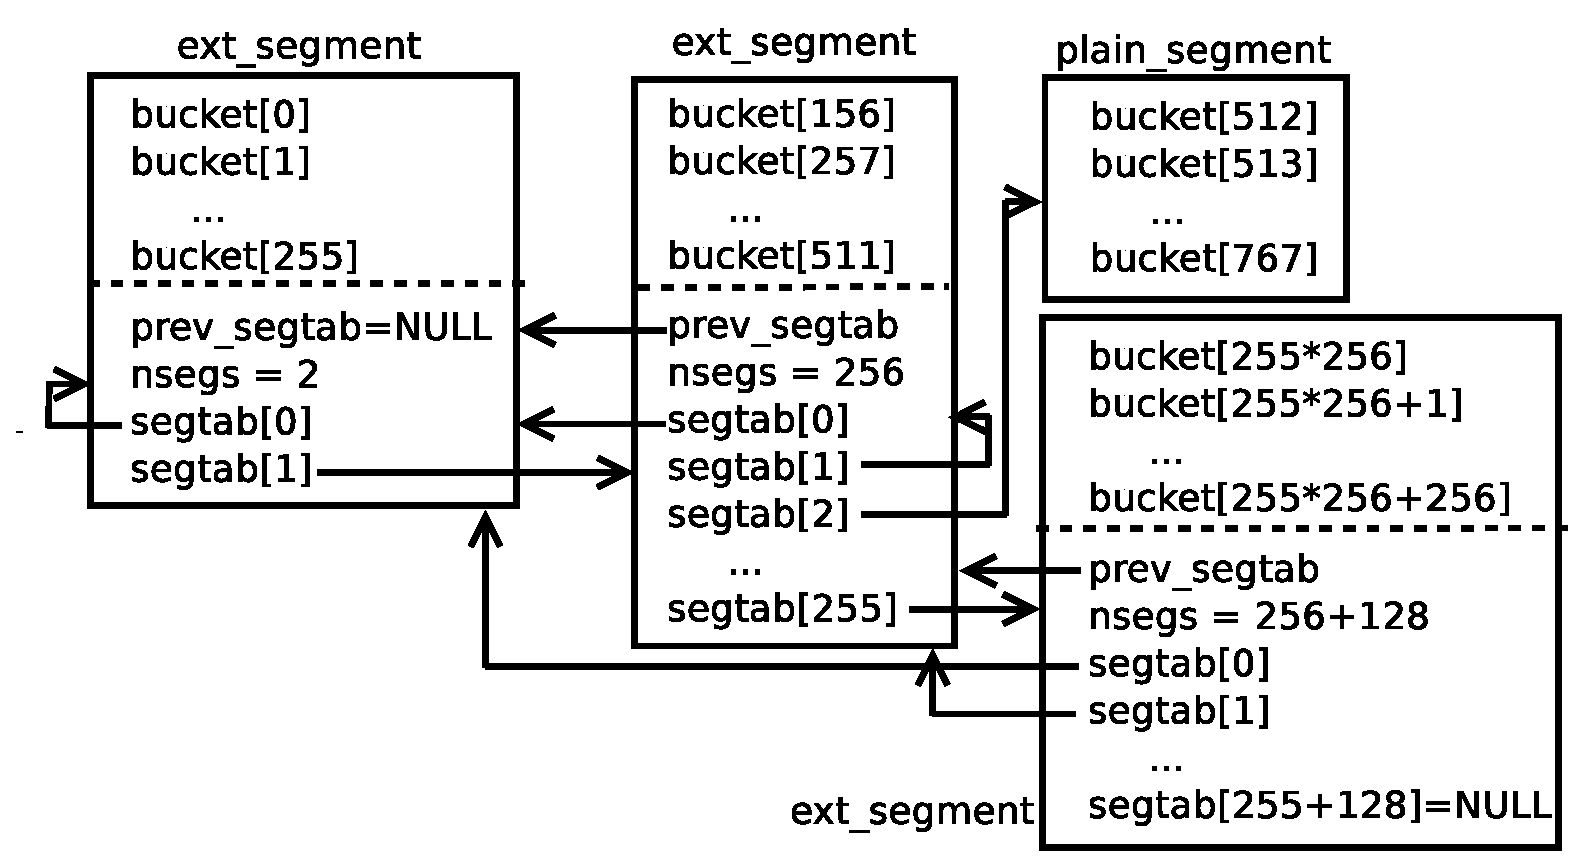
\includegraphics[width=1.0\textwidth]{hash_table_structure.eps}
\caption{Hash table structure} 
\label{fig:hash_table_structure}
\end{figure}

\subsubsection{Growing}

Growing is triggered after table insertion, when the total number of entries in the table exceeds a predefined value.
Currently this value is set so that if a uniform distribution of objects is assumed, each bucket has a chain length of 6.
Growing happens by splitting a bucket, moving objects to the bucket after the one that is currently active.
The bucket to be split is the one at half the new bucket's index.
If the segment address of the new bucket corresponds to a slot in the index segment that is currently not pointing to a bucket section, a new plain bucket section is allocated and the slot is now pointing to its first entry.
If this operation would assign a slot in the last slot of the segment section of currently active extended segment, a new extended segment is allocated instead, with more slots in its segment section.
The first extended segment has 2 slots in its segment section.
The second extended segment has 256 slots in its segment section.
Each next extended segment has 128 more slots in its segment section than the previous.
After a new extended segment is allocated, all the pointers from the segment section of the old extended segment are copied into the low slots of the segment section of new extended segment.
This leads to duplication (the same plain bucket sections are accessible from multiple extended segment sections), but enables reaching the contents of a bucket by using the segment section of just the current extended segment.
The new extended segment does not immediately replace the old one.
This happens when yet another segment must be allocated.
(This will be a plain segment, stored in the segment section of the new extended segment.)

\subsubsection{Shrinking}

Shrinking may happen after deletion, if the total number of entries falls below a predefined value.
Shrinking works in the reverse direction of growing:
The active bucket with the highest index is merged with its corresponding ``low'' bucket.

Shrinking might lead to the deallocation of a plain or extended bucket segment, if none of the buckets in it is active.
Once the first bucket not accessible through the previous extended segment is deallocated, the previous extended segment is restored as current extended segment.
This happens in order to avoid deallocating an extended segment while its segment table may still be used by other threads.
When the extended segment is later deallocated, the contents of all the buckets in the bucket section have been rehashed, seizing *all* locks, so there cannot exist any processes still executing code using the old extended segment pointer.
For this to work, we must of course allocate a new extended segment one call earlier.
This is also the reason why the minimum size of the first segment table is 2 and not 1 (NSEG\_1).

\subsubsection{Hash table types}     % section 2.1

With the underlying implementation being the same for all the types of hash tables, the specific type of the table introduces only minor differences in specific operations.

\paragraph{Set}

Insertion in tables of \verb|set| type should overwrite the existing value.
It should also fail if the insertion is performed with a insert\_new operation.

\paragraph{Bag, Duplicate Bag}

Special care should be taken to include/skip keys with the same value.

\subsection{Ordered Set table type}

The ordered set table type is implemented with an AVL tree.
There exists no fine locking.

\section{Concurrency Options} \label{sec:concurrency_options}

Read and write concurrency are orthogonal:
write concurrency adds finer-level locks that can be used to read or write to particular sets of objects in the table, while read concurrency changes the type of all the locks used by the table.

\subsection{Write Concurrency}

The addition of finer-level locks is done only on hash-based tables that have either protected or public access rights.
More details are provided in the relevant section.

\subsection{Read Concurrency}

[Changes mutex\_normal to mutex\_freq\_read]

\section{Fixation}

A process can call \texttt{ets:safe\_fixtable(Table, true $|$ false)} to put a fixation on a table implemented with a hash table (\verb|set|, \verb|bag| or \verb|duplicate_bag|).
When a table is fixed, a sequence of \verb|first/1| and \verb|next/2| calls are guaranteed to succeed and each object in the table will only be returned once, even if objects are removed or inserted during the traversal.
The keys for new objects inserted during the traversal may be returned by \verb|next/2| (it depends on the internal ordering of the keys).
In practice, this translates to the following 2 guarantees:

\begin{enumerate}
  \item Keys will not totally disappear from the table.
    A key can thus be used as an iterator to find the next key in iteration sequence.
    Note however that this does not mean that (pointers to) table objects are guaranteed to be maintained while the table is fixated.
    A BAG or DBAG may actually remove objects as long as there is at least one object left in the table with the same key (alive or pseudo-deleted).
    \item Objects will not be moved between buckets due to table grow/shrink.
      This will guarantee that iterations do not miss keys or get double-hits.
\end{enumerate}

\subsection{Implementation}

Fixation is monitored by a flag on the table itself and a mapping between PIDs and the identifiers of the tables that the respective process has fixated.
The fixation flag is checked before growing or shrinking a table to make sure that possible split or merges won't lead into duplicate appearance of objects in a traversal.
Objects on a fixed table are not deleted if there exist no other objects with the same key.
Instead objects are marked with an ``invalid\_hash'' flag and added to a list with objects that must be deleted after the fixation has been lifted.

\section{Benchmark} \label{sec:benchmark}

  A simple benchmark has been performed.
  The purpose of the benchmark is to see how the \verb|write_concurrency| and \verb|read_concurrency| options affect the performance of different table types on a real world problem.
  The benchmark creates workers that all do \verb|lookup|s and \verb|insert|s on the same ETS table.
  The benchmark was done on a computer with 64 cores.
  The benchmark was run with all combinations of \verb|write_concurrency| and \verb|read_concurrency| together with the table types \verb|set| and \verb|ordered_set|.
  
  \subsection{Benchmark Problem}
    The benchmark program finds the minimum number of sort steps to sort an array.
    The array contains \emph{black} marks, \emph{white} marks and \emph{empty} positions.
    The sequence \verb|"ebbwe"| can represent an array, where an \verb|e| represent an \emph{empty} position, a \verb|w| represent a \emph{white} mark and an \verb|b| represents a \emph{black} mark.
    Black marks can only move towards the right end of the array and white marks can only move towards the left end.
    In one sort step a mark can:
    \begin{itemize}
     \item move one step in the array if the neighbor position in the direction of the movement is empty or
     \item move two steps in the array if the neighbor position in the direction of the movement contains a mark and the position after the neighbor position is empty.
    \end{itemize}
    A sorted array has all white marks as far to the left in the array as possible and all black marks as far to the right in the array as possible.
    Some input arrays can not be sorted with the given constraints, e.g. \verb|"bbww"|.
    If the input array can not be sorted the program shall return $-1$.
    For example the minimum number of steps for \verb|"ebbwe"| is $5$.
    The benchmark timed the time it took to return the result for the arrays \verb|"bebebbeeeewwwbw"|, \verb|"bebebeeewewewewwe"|.
    
  \subsection{Implementation}
    The Erlang program that solves the benchmark problem is available at www.github.com\footnote{http://github.com/kjellwinblad/ets\_impl\_project/blob/master/benchmark/multi\_4.erl}.
    The program explores the the possible solutions using breadth first search.
    Explored configurations are saved in an ETS table to avoid repeating work.
    
    The program has one coordinator process and a number of worker processes.
    At a specific level in the search tree, the coordinator divides the configurations that needs to be explored in the next level evenly and sends them to the workers.
    The workers send a message to the coordinator if a solution is found.
    If a worker finds a configuration that is not a solution, it is expanded by generating all possible configurations that can be created by performing one sort step.
    
    Directly after a configuration is generated, it is checked whether it already exists in the ETS table cache with the \verb|ets:member| function.
    If it already exists, it is thrown away because the configuration has already been visited.
    Otherwise, the configuration is inserted in the ETS table with the \verb|ets:insert_new| operation.
    The return value of \verb|ets:insert_new| is checked to make sure that the configuration has not been inserted by another process between the call to \verb|ets:member| and \verb|ets:insert_new|.
    The Erlang code that is interacting with the ETS table cache in the workers can be seen in listing~\ref{li_erlang_ets_interaction}.

    \lstset{language=erlang, caption=Worker code that is interacting with ETS, label=li_erlang_ets_interaction} 
\begin{lstlisting}[float=htb] 
IsFound = ets:member(Cache, MoveArray),
case IsFound of
  false ->
    Inserted = ets:insert_new(Cache, {MoveArray}),
    case Inserted of
      true ->
        [MoveArray|all_next_step_arrays(Array, CurrentPos + 1, Cache)];
      false ->
        all_next_step_arrays(Array, CurrentPos + 1, Cache)
    end;
  true ->
    all_next_step_arrays(Array, CurrentPos + 1, Cache)
end
\end{lstlisting}
    
    A worker sends back all the configurations that needs to be explored in the next level to the coordinator, when it has processed all given configurations on the current level.


\subsection{Results}

  The results of the benchmark can be seen in figure~\ref{fig:benchmark_results}.
  The filled straight line labeled \emph{serial} is the performance of a serial version of benchmark program.
  The serial version can also be found at www.github.com\footnote{http://github.com/kjellwinblad/ets\_impl\_project/blob/master/benchmark/single\_1.erl}.
  The graphs with \emph{set} in the label show the benchmark times for the table type \verb|set|.
  The graphs with \emph{ordset} in the label show the benchmark times for the table type \verb|ordered_set|.
  A \emph{w} in the label means that the table has \verb|write_concurrency| enabled and an \emph{r} in the label means that the table has \verb|read_concurrency| enabled.
  
  
\begin{figure}[htb]
\centering
\includegraphics[width=1.0\textwidth]{benchmark.eps}
\caption{Benchmark Results} 
\label{fig:benchmark_results}
\end{figure}

  The table type \verb|set| with \verb|write_concurrency| enabled seems to give similar performance both with and without \verb|read_concurrency| enabled.
  All other configurations give similar performance to each other.
  It is not surprising that all \verb|ordered_set| configurations perform similarly since the \verb|write_concurrency| and \verb|read_concurrency| options do not affect this table type at all.
  The \verb|ordered_set| table type should theoretically have more expensive \verb|lookup| and \verb|insert| operations compared to the \verb|set| table type.
  This does not seem to have any significant effect on this benchmark.
  
  In this particular benchmark it seems like \verb|write_concurrency| for the table type \verb|set| is particularly important for scalability.
  For the other configurations the performance seems to get worse, when more than five worker processes are used.
  It is reasonable to assume that the reason for this is that the contention become higher when the number of workers is increased.

  
  
\section{Scalable ETS Suggestions}

  The benchmark that is described in section~\ref{sec:benchmark}, shows that the fine grained locking provided by the \verb|write_concurrency| option can be very important for scalability.
  The number of locks used when fine grained locking is enabled is hard coded to 16 in the current implementation.
  It is tempting to make the locking even more fine grained, since it could possibly make ETS more scalable.
  However, it might increase processor cache misses and have other unforeseen effects so it is not certain that it will give better scalability. 
  
  The benchmark described in section~\ref{sec:benchmark} has also been run with a versions of the runtime environment with the number of locks set to 32 and 64.
  This change did not seem to have any significant effect on the performance of the benchmark program.
  There might be other bottleneck in this particular benchmark that are more important.
  It would be interesting to look more deeply into how the number of locks effect the performance on other benchmarks.
  
  The benchmarks of Judy-array based ETS table implementations that are described by Fritchie, suggests that there are other table implementations that are significantly faster than the current ones for some use cases~\cite{ScottEtsJudy}.
  Fritcie did not discuss how to make the Judy-array based ETS table implementation concurrent.
  Prokopec, Bagwell and Odersky have described a ''lock-free'' concurrent data type called CTrie which is similar to the ETS table implementation suggested by Fritcie~\cite{ProkopecCTrie}.
  Benchmarks indicate that CTries scales well compared to many other concurrent table implementations~\cite{ProkopecCTrie}.
  Adding a CTrie data type as an Erlang ETS table type could potentially provide better scalability than the current implementation.
  
  The current ETS table implementation has no good support for use cases when more than one table operation need to be performed atomically.
  The only practical way to support that use case with the current ETS implementation is to serialize all access to the ETS table or ETS tables involved.
  Transactional support for ETS tables as suggested in~\cite{PatrikErlangTrans} could be a way to support this use case in a much more scalable way.
  
  In the current implementation of ETS, all terms that are inserted or fetched from an ETS table are copied from or to the ETS table.
  This might be expensive both in respect to time and memory if many processes access the same objects in the table.
  An alternative would be to use references for terms that are stored in ETS tables. 
  The Erlang runtime already uses references for large values of the binary data type.
  Therefore, it might be possible to reuse some existing components in the Erlang runtime system, to implement references for terms stored in the ETS tables with some potential performance benefits.
  
  The current \verb|ordered_set| table type uses only one lock for the whole data structure. 
  There exist implementations of binary trees that scale much better than the current \verb|ordered_set| implementation and that have support for efficient traversal of the tree.
  Bronson, Casper, Chafi and Olukotun have described a relaxed AVL-tree data-structure with STM inspired methods for thread safety~\cite{BronsonPracTree}.
  This implementation could give much better scalability on a multi-core computer than the current \verb|ordered_set| implementation.
  

\bibliographystyle{unsrt}  

\bibliography{report}
  

\end{document}
